\clearpage
\section*{Agradecimientos}
\par Me gustaría darle las gracias a Richard Stallman \cite{stallman} y todas las personas que han colaborado con la {\em Free Software Foundation} \cite{fsf}.
\par También le doy las gracias a Donald Knuth \cite{knuth} y a todas las personas que han ayudado a crear TeX \cite{tex} y sus increíbles macros.

\chapter{Introducción}
\par En los últimos años, la mayoría de los ataques en Internet se realizan contra aplicaciones web, con lo que es cada vez más importante contar con una
solución que sea capaz de analizar el tráfico web y proteger estas aplicaciones.
\par Y, no importa el proceso de desarrollo, no importa el número o la calidad de los controles de seguridad desplegados, no existe una aplicación completamente
segura; tal como afirma el adagio:

\say{La seguridad 100\% no existe.}

\par Con este punto de partida, y teniendo en cuenta el uso masivo que las aplicaciones hacen del Protocolo de transferencia de hipertexto (en adelante
\acrshort{http}, de sus siglas en inglés \acrlong{http}) y del Protocolo seguro de transferencia de hipertexto (en adelante \acrshort{https}, de sus siglas en
inglés \acrlong{https}), es inmediato identificar por qué la mayoría de los ataques actuales se realizan contra aplicaciones publicadas a través de estos
protocolos.

\par Para protegerlas existen múltiples mecanismos de seguridad, desde herramientas que monitorizan el uso indebido de datos como el Software de prevención de
pérdida de datos (en adelante \acrshort{dlp}, de sus siglas en inglés \acrlong{dlp}), herramientas de red como son el firewall tradicional o herramientas más
dirigidas como son los firewall de aplicación web (en adelante \acrshort{waf}, de sus siglas en inglés \acrlong{waf}).

\par En entornos con una gran infraestructura, que generen una facturación importante o con un alto riesgo, es habitual que se desplieguen las herramientas
mencionadas y muchas otras, incluso herramientas redundantes siguiendo el principio de \gls{DefensaProfundidad}, que aboga por desplegar múltiples sistemas
de protección con el fin de que si uno falla otro pueda detener el ataque.
\par Pero, en entornos en los que los recursos son más limitados, no es viable desplegar todos los controles de seguridad que serían deseables. Por recursos no
sólo se entiende económicos, sino también por personas con el tiempo, el conocimiento y la experiencia como para desplegar y mantenerlas.
\par En estos entornos es habitual que los controles de seguridad se limiten a un firewall de red o, si se dispone de algo más de presupuesto, un sistema de
Gestión Unificada de Amenazas (más conocido como \acrshort{utm}, de sus siglas en inglés \acrlong{utm}~\cite{wiki:utm}).
\par Este tipo de soluciones no son capaces de ofrecer una protección adecuada contra ataques en capa de aplicación. Por ejemplo, los firewall tradicionales son
capaces de analizar el tráfico de red en capa 3 del modelo TCP/IP\cite{wiki:tcpip} (equivalente a las capas 3 y 4 del {\em modelo OSI\cite{osi}}). Esto implica que, cuando se
publica un servicio web, dichos firewall permitirán todo el tráfico dirigido a estos servicios, con independencia de que se trate de una petición legítima, una
petición incorrectamente formada o un ataque.
\par Para proteger estos servicios web adecuadamente es necesario disponer de tecnologías con capacidad de analizar el tráfico en la capa de aplicación
siguiendo la lógica propia del servicio a proteger, como los mencionados WAF.

\par Otro aspecto que se debe tener en cuenta consiste en la migración constante que se está produciendo de forma generalizada de tráfico sin cifrar - también
conocido como en texto plano - a tráfico cifrado HTTPS en el que se encapsula el tráfico HTTP en un canal \acrshort{ssl}/\acrshort{tls}
(\acrlong{ssl}/\acrlong{tls} respectivamente~\cite{wiki:ssltls}). Históricamente se utilizaban múltiples herramientas perimetrales como son los sistema de
detección de intrusiones (en adelante \acrshort{nids}, de sus siglas en inglés \acrlong{nids}) o los mencionados firewall. Una de las limitaciones que tienen
este tipo de herramientas es que no participan en la negociación SSL/TLS, por lo que no son capaces de descifrar el tráfico y no pueden analizar el contenido de
las peticiones o sus respuestas. Estas herramientas son, por lo tanto, cada vez menos efectivas a la hora de detectar y bloquear amenazas, pues carecen de la
visibilidad adecuada en un gran porcentaje del tráfico.
\par Por último, se debe considerar otro cambio significativo que se está produciendo en estos últimos años: Cada vez es más habitual desplegar las aplicaciones
en \gls{cloud} (o Cloud, se utilizarán ambos términos indistintamente debido a lo extendido de ambos términos). En estos entornos se diluyen los conceptos de
red perimetral o segmentación de red y es más complejo desplegar controles de seguridad perimetrales como los mencionados firewall, NIDS o UTM. En estos
entornos muchos de los componentes de la infraestructura son transparentes para el cliente y no es posible desplegar mecanismos en estas capas.
\par A modo de referencia, en la tabla {~\hyperref[fig:Responsabilidadescloud]{Responsabilidades compartidas en el Cloud}} vemos como los únicos elementos sobre
los que se mantiene el control en los distintos modelos del Cloud son la capa de aplicación y los datos (con la excepción del modelo de Software como un
Servicio, en adelante \acrshort{saas}, de sus siglas en inglés \acrlong{saas}).
\begin{figure}[hp]
  \centering
  \label{fig:Responsabilidadescloud}
  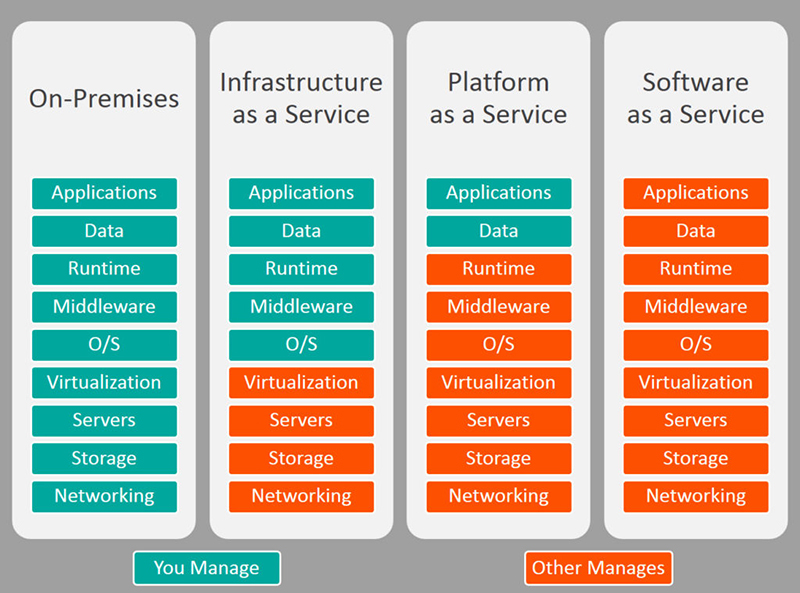
\includegraphics[width=0.7\textwidth]{fig/Responsabilidadescloud}
  \caption{Responsabilidades compartidas en los modelos Cloud (fuente MR Informática~\cite{Responsabilidadescloud}).}
\end{figure}

\par Es por lo tanto, cada vez más importante contar con herramientas que sean capaces de descifrar y analizar el tráfico HTTPS y, según se verá con más detalle
en la sección ~\nameref{subsec:estadoarte}, estas soluciones implican o bien un desembolso económico significativo en el caso de las soluciones privativas o
bien se despliegan como módulos de la propia aplicación web en las soluciones de {\em software libre\cite{softwarelibre}}.
\par En este segundo grupo, las soluciones requieren un ejercicio de integración con las aplicaciones web y consumen recursos del servidor que pueden impactar
en el rendimiento. Adicionalmente, para la implementación y configuración adecuada de estos módulos se requiere de una persona con un conocimiento profundo de
la seguridad de aplicaciones web que se mantenga informado de las últimas novedades del sector y que administre y actualice el entorno según se detectan nuevos
ataques y mecanismos paliativos.  Debido a estos factores y la complejidad que el WAF añade a la plataforma web, es habitual que cuando una plataforma web
requiere de una actualización importante o una migración de tecnologías, el modulo de WAF se desactive o elimine completamente.

\par Como respuesta a esta necesidad surge el presente proyecto, cuyo objetivo es construir una solución de software libre con capacidades de WAF, aceleración
SSL/TLS, fácilmente desplegable y que minimice el esfuerzo y el impacto que dicha solución tiene sobre la plataforma web actual o futura.
